\documentclass[12pt]{extarticle}
\usepackage{tempora}
\usepackage[T1, T2A]{fontenc}
\usepackage[utf8]{inputenc}
\usepackage[english, ukrainian]{babel}
\usepackage{geometry}
\usepackage{graphicx}
\usepackage{multirow}
\usepackage{multicol}
\usepackage{float}
\graphicspath{{/home/artem/Pictures}}
\geometry
{
    a4paper,
    left=30mm,
    top=15mm,
    right=20mm,
    bottom=15mm,
}

\begin{document}
\begin{titlepage}
    \begin{center}
        \textbf{\normalsize{\MakeUppercase{
            Міністерство Освіти і науки України
            Національний університет "Львівська політехніка"
        }}}

        \begin{flushright}
        \textbf{ІКНІ}\\
        Кафедра \textbf{ПЗ}
        \end{flushright}
        \vspace{15mm}

        \includegraphics[width=0.4\textwidth]{lpnu_logo.png}

        \vspace*{\fill}

        \textbf{\normalsize{\MakeUppercase{Звіт}}}
            
        До лабораторної роботи №2

        \textbf{на тему:} “МОДЕЛЮВАННЯ ТА ДОСЛІДЖЕННЯ ОСНОВНИХ ТИПІВ ТРИГЕРІВ В
СИСТЕМІ PROTEUS”

        \textbf{з дисципліни:} “Архітектура комп’ютера”
            
        \vspace*{\fill}

        \begin{flushright}

            \textbf{Лектор:}\\
            доцент кафедри ПЗ\\
            Крук О.Г.\\
            \vspace{12pt}

            \textbf{Виконав:}\\
            студент групи ПЗ-24\\
            Губик А. С.\\
            \vspace{12pt}

            \textbf{Прийняв:}\\
            доцент кафедри ПЗ\\
            Задорожний І. М.\\
        \vspace{12pt}
        \end{flushright}

        Львів -- 2023
            
            
    \end{center}
\end{titlepage}

\textbf{Тема роботи:} моделювання та дослідження основних типів тригерів в 
системі Proteus

\vspace{12pt}

\textbf{Мета роботи:} закріпити практичні навики моделювання логічних схем в
середовищі системи програм Proteus; поглибити знання про
будову та функціонування основних типів тригерів; ввести їх
схеми та виконати моделювання в системі програм Proteus;
дослідити на основі отриманих часових діаграм їх роботу.

\subsection*{Індивідуальне завдання}
\begin{center}
    \begin{tabular}{| c | c | c |}
        \hline
        \multicolumn{2}{|c|}{Варіант 3}\\
        \hline
        $f_0$, КГц & 15\\
        \hline
   
    \end{tabular}
\end{center}

\subsection*{Теоретичні відомості}
Тригер – це електронний вузол з двома стійкими станами, зміна яких
відбувається під дією вхідних сигналів. Якщо прийняти один стан тригера за
логічний нуль, а інший – за логічну одиницю, то виходить, що тригер є елементом
пам’яті, який може зберігати один біт інформації. Тригер є найпростішим
представником послідовнісних пристроїв і водночас обов’язковим елементом всіх
функціонально закінчених вузлів і блоків.
У послідовнісних пристроях (цифрових автоматах з пам’яттю або скінченних
автоматах) вихідні сигнали в кожний момент часу залежать не лише від поточних
значень на входах, але й від внутрішнього стану, який є наслідком попередніх дій
вхідних сигналів.
На основі тригерів будують типові функціональні вузли комп’ютерів –
регістри, лічильники, накопичувальні суматори, а також мікропрограмні автомати.
Усі різновиди тригерів можна розглядати як елементарний автомат, що
складається з власне елемента пам’яті (ЕП) та схеми керування (СхК), яка утворює
вхідну логіку (рис. 3.1). Схема керування забезпечує записування, зчитування,
стирання та індикацію двійкової інформації, яка зберігається в тригері.
При позитивному кодуванні інформації високий рівень напруги на прямому виході
відображає значення логічної 1 (стан Q =1), а низький рівень – значення логічного
0 (стан Q = 0). Сигнали на виходах тригера в усталеному режимі завжди повинні
бути протилежними: якщо на прямому виході є одиниця, то на інверсному - 0, або
навпаки.
Зміна стану тригера (його перемикання) забезпечується зовнішніми сигналами
та сигналами зворотного зв’язку з виходу тригера, які поступають на входи СхК.
Переважно зовнішні сигнали, як і входи тригера, позначають латинськими буквами
R, S, Т, С, V та іншими. В найпростіших схемах тригерів окрема СхК може бути
відсутньою.
Оскільки функціональні властивості тригерів визначаються їхньою СхК, то
назви основних входів переносяться на всю схему тригера.
Назва “RS-тригер” утворена від перших літер слів RЕSЕТ (скинення –
занесення нуля) і SЕТ (установлення- занесення одиниці ).
Схема RS-тригера на двох послідовно з’єднаних логічних елементах АБО-НЕ
наведена на рис. 3.2, а. Визначальним в роботі цього тригера є додатний зворотний
зв’язок – сигнал з виходу другого (нижнього) елемента АБО-НЕ подається на вхід
першого (верхнього) елемента АБО-НЕ. Саме завдяки додатному зворотному
зв’язку тригер має два стійких стани. На рис 3.2, б наведено умовне графічне
позначення RS-тригера на електричних схемах.
\subsection*{Хід роботи}
\paragraph{1.}x

\vspace{12pt}
\begin{figure}[H]
    \centering
    \includegraphics[width=0.90\textwidth]{nand_triger.jpg}
    \caption{RS-тригер на елементах NAND}
\end{figure}
\begin{figure}[H]
    \centering
    \includegraphics[width=0.90\textwidth]{nand_triger_graph.jpg}
    \caption{Графік}
\end{figure}

\paragraph{2.}x
\begin{figure}[H]
    \centering
    \includegraphics[width=0.90\textwidth]{nor_triger.jpg}
    \caption{RS-тригер на елементах NOR}
\end{figure}
\begin{figure}[H]
    \centering
    \includegraphics[width=0.90\textwidth]{nor_triger_graph.jpg}
    \caption{Графік}
\end{figure}

\vspace{12pt}

\paragraph{3.}x

\begin{figure}[H]
    \centering
    \includegraphics[width=0.90\textwidth]{sync_rs.jpg}
    \caption{Синхронний RS-тригер}
\end{figure}
\begin{figure}[H]
    \centering
    \includegraphics[width=0.90\textwidth]{sync_rs_graph.jpg}
    \caption{Графік}
\end{figure}
\paragraph{4.}x
\begin{figure}[H]
    \centering
    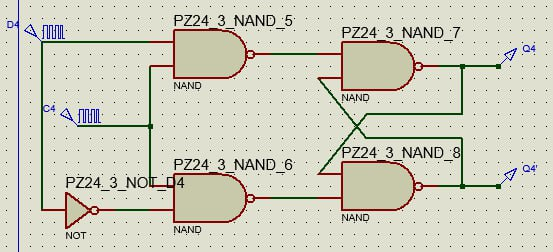
\includegraphics[width=0.90\textwidth]{d_triger.jpg}
    \caption{Синхронний D-тригер}
\end{figure}
\begin{figure}[H]
    \centering
    \includegraphics[width=0.90\textwidth]{d_triger_graph.jpg}
    \caption{Графік}
\end{figure}
\paragraph{5.}x
\begin{figure}[H]
    \centering
    \includegraphics[width=0.90\textwidth]{jk.jpg}
    \caption{Синхронний JK-тригер}
\end{figure}
\begin{figure}[H]
    \centering
    \includegraphics[width=0.90\textwidth]{jk_graph.jpg}
    \caption{Графік}
\end{figure}
\paragraph{6.}x
\begin{figure}[H]
    \centering
    \includegraphics[width=0.90\textwidth]{jk+.jpg}
    \caption{D-тригер на основі JK-тригер}
\end{figure}
\begin{figure}[H]
    \centering
    \includegraphics[width=0.90\textwidth]{jk+graph.jpg}
    \caption{Графік}
\end{figure}
\paragraph{7.}x
\begin{figure}[H]
    \centering
    \includegraphics[width=0.90\textwidth]{jk_active.jpg}
    \caption{Інший JK-тригер}
\end{figure}
\begin{figure}[H]
    \centering
    \includegraphics[width=0.90\textwidth]{jk_active_graph.jpg}
    \caption{Графік}
\end{figure}
\paragraph{8.}x
\begin{figure}[H]
    \centering
    \includegraphics[width=0.90\textwidth]{t_triger.jpg}
    \caption{D-тригер на основі JK-тригер}
\end{figure}
\begin{figure}[H]
    \centering
    \includegraphics[width=0.90\textwidth]{t_triger_graph.jpg}
    \caption{Графік}
\end{figure}

\textbf{Висновок:} Я дізнався які є види тригерів і як вони працюють.


\end{document}